\documentclass[20pt,a1paper,landscape,blockverticalspace=-0.25in]{tikzposter}
\usepackage[utf8]{inputenc}
\usepackage{csquotes}
\usepackage{amsmath}
\usepackage{amsfonts}
\usepackage{amsthm}
\usepackage{amssymb}
\usepackage{mathrsfs}
\usepackage{graphicx}
\graphicspath{{./images/}}
\usepackage{adjustbox}
\usepackage{enumitem}
\usepackage{xcolor}
\usepackage{tartu}
\usepackage{bm}
\usepackage[comma]{natbib}
\usepackage{har2nat}
\bibliographystyle{agsm}
\setcitestyle{citesep={;}}
\renewcommand{\bibsection}{}
\setlength{\bibsep}{0pt}

% set theme parameters
\tikzposterlatexaffectionproofoff
\usetheme{UniTartuTheme}
\usecolorstyle{UniTartuStyle}

\usepackage[scaled]{helvet}
\renewcommand\familydefault{\sfdefault} 
\renewcommand{\vec}[1]{\bm{#1}}
\newcommand{\Tr}{\text{Tr}}
\usepackage[T1]{fontenc}
\usepackage[hidelinks]{hyperref}
\title{Bayesian Inference of Parameters for Numerical Storm Surge Models}
\author{\textbf{Benjamin Russell}\textsuperscript{1}}
\institute{\textsuperscript{1}University of Durham\\}
\titlegraphic{
\includegraphics[width=0.12\linewidth]{logo.png}}

% begin document
\begin{document}
	\maketitle
	\centering
	\begin{columns}
		\column{0.32}
		\block{Background}{
			In the United States of America coastal communities suffer huge yearly losses from flooding. One of the causes of such flooding is storm surges, this is the sea level rise caused by tropical hurricanes and cyclones. Studies have shown that between 1963 and 2012 49\% of all deaths from hurricanes in the US were caused by the storm surge(Fig. \ref{fig:deaths})~\cite{deaths}. The economic impact has also been huge with estimates showing that with no further improvements to coastal flood defenses by 2050 yearly losses from storm surge flooding could exceed US\$1trillion~\cite{costs}.
			
			Following this it makes sense to model and simulate these storm surge events to facilitate better planning for flood defence spending. Most storm surge models require finely tuned parameters which either requires direct measurement which can be expensive and difficult to carry out or to be inferred from previous data. Inferrence of these parameters requires huge numbers of time consuming model runs. To address this we investigate the use of various surrogate models that approximate the model outputs in much less time so this inferrence can be carried out. We focus on the coefficients of friction at varying water depths as our parameters.
		}
		\block{Aims and Objectives}{
			\begin{itemize}[itemsep=-0.25ex]
				\item
				Implement a storm surge model using GeoClaw~\cite{clawpack,mandli2016clawpack,geoclaw}
				\item
				Implement and use the kriging surrogate modelling method to infer friction parameters
				\item
				Implement Polynomial Chaos Expansion (PCE)  as a surrogate method to infer the friction parameters
				\item
				Implement the hybrid Polynomial Chaos Kriging (PC-Kriging) surrogate model as a hybrid to infer the friction parameters.
				\item
				Analyse the inferred parameters from each surrogate model and compare the accuracy when used in the full model, as well as the uncertainty in the approximations.
			\end{itemize}
		}
	
		\column{0.36}
		\block{Causes of Hurricane Deaths}{
			\begin{tikzfigure}[Deaths in the US caused by hurricanes between 1963-2012~\cite{deaths}\label{fig:deaths}]
				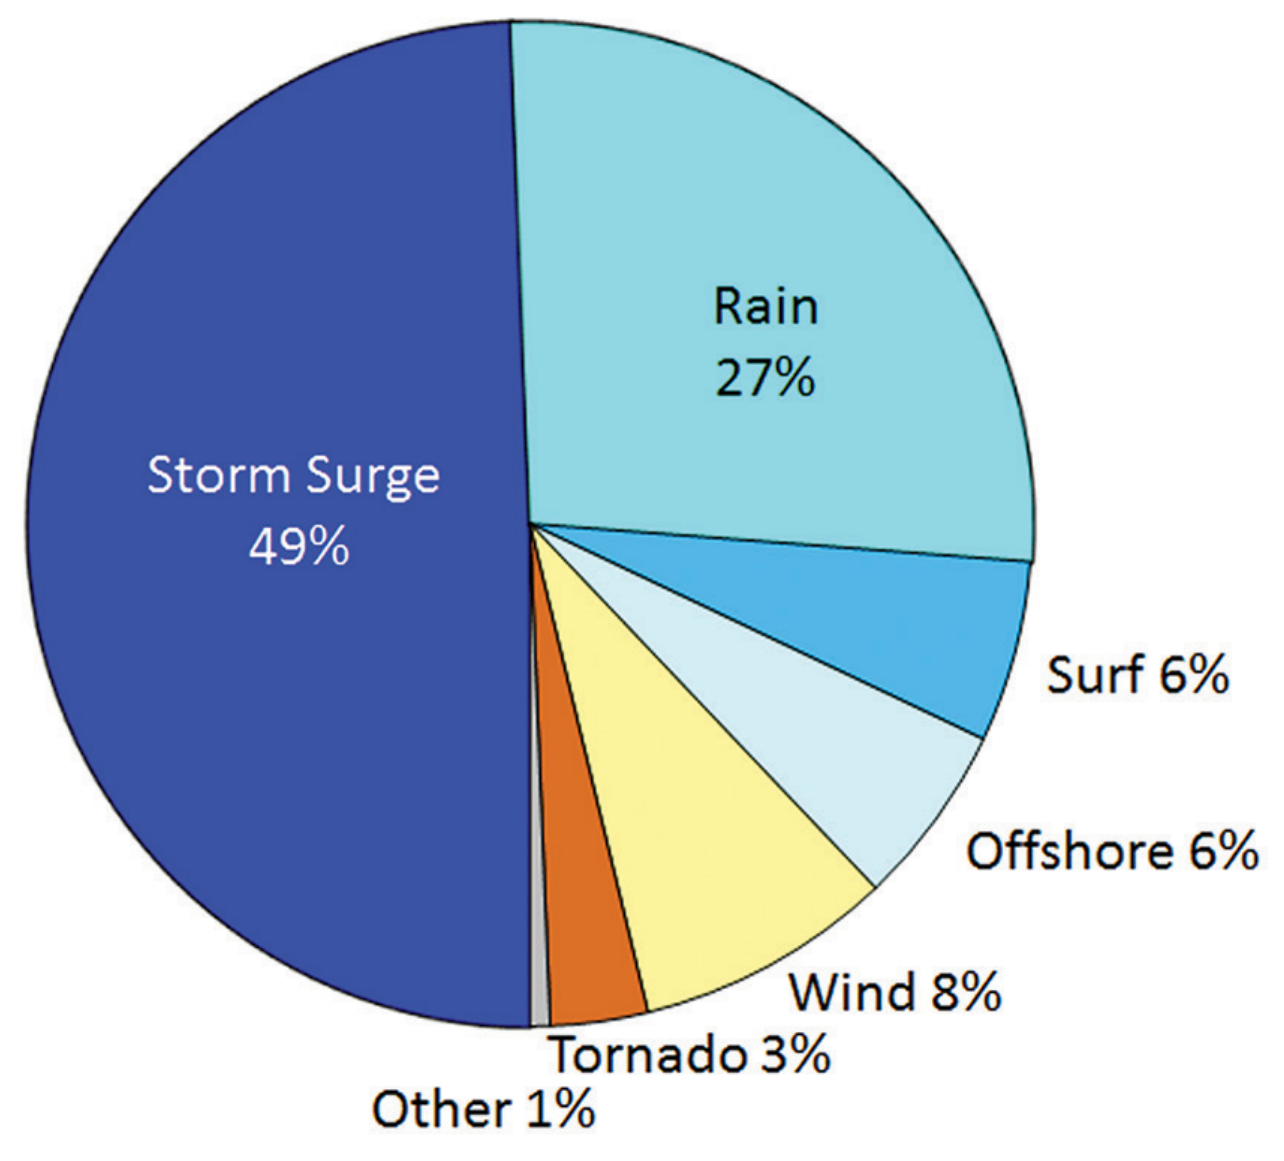
\includegraphics[width=0.5\linewidth]{Deaths}
			\end{tikzfigure}
		}
		\block{Method}{
			\begin{itemize}[itemsep=-0.25ex]
				\item
				Formulate the parameter inferrence problem as an instance of Bayesian inferrence:
				\begin{gather*}
					P(n_1,n_2,n_3,\sigma^2_i|\eta_i)\propto L(\eta|n)q(\sigma^2)q(n_1)q(n_2)q(n_3) \\
					L(\eta|n) = \frac{1}{\sqrt{2\pi\sigma^2}}\prod_i\exp\left(
					\frac{-(\eta_i - M_i(n))^2}{2\sigma^2}
					\right)
				\end{gather*}
				$n_i$ represents friction parameters, $\eta_i$ represents actual observed sea level rise, $M_i$ is the model output for sea level rise, and $q(k)$ are prior distributions of model parameters.
				\item
				Using the formulation by repeatedly sampling from the posterior it is possible to infer the distribution of friction parameters. This sampling will be carried out using the Markov Chain Monte Carlo (MCMC) algorithm due to the multidimensionality of the problem.
				\item
				Updating and sampling from the posterior will be done cheaply by using the surrogate models rather than the GeoClaw model.
				\item
				After inferring the parameters with each surrogate model, they will be used with the GeoClaw model and their accuracies compared when simulating the resulting storm surge from Hurricane Ike (2008).
			\end{itemize}
		}
		
		\column{0.32}
		\block{Surrogate Models}{
			\begin{itemize}[itemsep=-0.25ex]
				\item
				The kriging surrogate is defined as~\cite{phd}:
				\begin{gather*}
					\bm{f_*}|\bm{f}\sim \mathcal{N}(\bm{\mu}_* + \Sigma_*^T\Sigma^{-1}(\bm{f}-\bm{\mu}),
					\Sigma_{**}-\Sigma_*^T\Sigma^{-1}\Sigma_*) \\
					\bm{\mu} = g(\bm{X})^T\cdot \bm{\beta} \\
					\bm{\mu}_* = g(\bm{X}_*)^T\cdot \bm{\beta}
				\end{gather*}
			\item
			The PCE surrogate is defined as~\cite{tsunami}:
			\begin{equation*}
				U(\bm{x},t,\zeta)=\sum_{k=0}^{P}U_k(\bm{x},t)\Psi_k(\zeta)
			\end{equation*} 
			\item
			The PC-Kriging model is based on that of~\citeasnoun{pckriging}, it is identical to the kriging model except that:
			\begin{equation*}
				\bm{\mu} = \sum_{k=0}^{P}U_k(\bm{x},t)\Psi_k(\zeta)
			\end{equation*}
			\end{itemize}
		}
		
		\block{Validity}{
			The proposed methodology is valid as the surrogates are closely based of off models used in the literature to solve similar hydrodynamic problems. The data shown in Fig. \ref{fig:deaths} demonstrates that this is an important problem to solve and the necessity of using surrogate models to do so is presented by \citeasnoun{tsunami}.
		}

		\block{References}{
			\vspace{-1em}
			\begin{footnotesize}
				\bibliography{refs}
			\end{footnotesize}
		}
	\end{columns}
\end{document} 
